\documentclass{article}
\usepackage{amsmath}

% Placeholder paragraphs with text
\usepackage{blindtext}

% figures
\usepackage{graphicx}

% No indent for new paragraphs
% \setlength\parindent{0pt}

% bibliography
\usepackage[
    backend=biber,
    style=bwl-FU,
    url=false,
    doi=false,
    eprint=false
]{biblatex}
\addbibresource{template-biblio.bib}

\begin{document}

\section{This is the highest level section header: some text}
\blindtext[1]

\subsection{This is a subsection: equations}

A simple equation:
\begin{equation}
x^2 + y^2 = 1
\end{equation}


% No indent for a single paragraph 
%\noindent
Multiple equations:
\begin{gather}
	x = 1 \\
	y = -1
\end{gather}



Aligned system of equations:
\begin{align}
\frac{\partial y}{\partial x} &= y ^ {\prime} (x) \\
\sum\limits_{i=1}^{N}y_i &= e^{\alpha + \beta x}
\end{align}

\subsubsection{Subsubsection is here: a figure}
Figure:

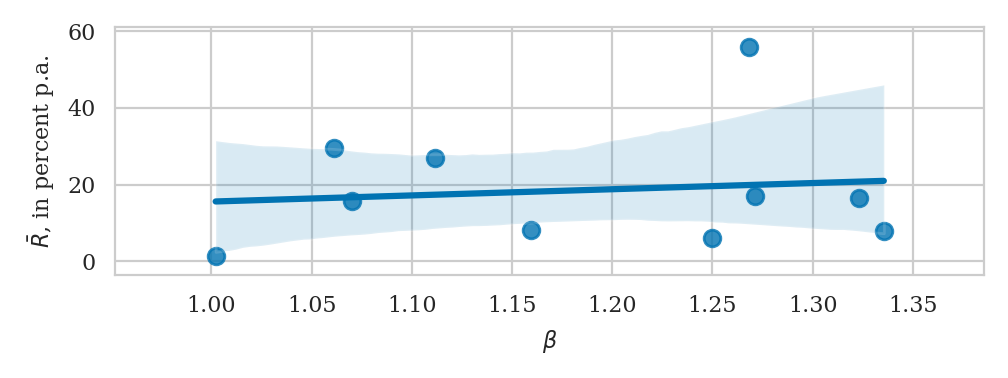
\includegraphics{../../figures/beta-vs-mu.png}

citation:
\cite{Cieslak2019}

\printbibliography

\end{document}
